\chapter{The Smartmedia Mobile News Recommender Use Case}

The use case following this thesis is the Smartmedia Mobile News Recommender system. The SMNRS is a program at the Department of Computer and Information Science at the Norwegian University of Science and Technology with a close collaboration with the Scandinavian media industry. It was established in 2012, and the program focuses on examining new technologies to help the news industry with the information overload situation and looking for ways to deliver news more efficiently and attractive to their readers.

The technologies essential to the SMNRS project are:

\begin{itemize}
	\item Big Data architectures
	\item Information retrieval and recommendation
	\item Semantics
	\item Text analytics and sentiment analysis
	\item Mobile platforms
\end{itemize}

\section{Client application}
As of now, there is only one client application making use of the SMNRS's back-end, which is an iOS application developed for iPhone running on iOS 6.0 and above. The client is developed as a part of this thesis and as a part of the SMNRS program. The iPhone client application's role in the whole project is shown in figure \ref{tech_news_app_architectural_view} and a video presenting the application can be found at \url{https://www.youtube.com/watch?v=3HgvnlqZ67A}.

\subsection{User Interface Design}
When the application is first launched, the user is met with a pop-up box where the user can agree or disagree to send the device's geoposition. Further the user is guided through an introduction phase showing how to use the application and which possibilities the app has. When this phase is completed, the user is met with the start screen with every application launch initiated from now on.

The start screen, as shown in the foremost image in figure \ref{screenshots_nyhetene_start_and_category}, shows the title of the latest recommended news article and how long it is since it was published. The title also works as a button and will reveal the corresponding article in the RSS view. In the top left corner it shows how many unread top stories there are, and in the top right corner the user has the ability to search for any topic or category it desires. Swiping to the right and releasing will trigger an update for the top stories, a swipe down will reveal the last read top story article, a swipe up will reveal the settings screen and a swipe to the left will reveal the category selection screen, as shown in the rear image in figure \ref{screenshots_nyhetene_start_and_category}.

\begin{figure}[!htbp]
\centering
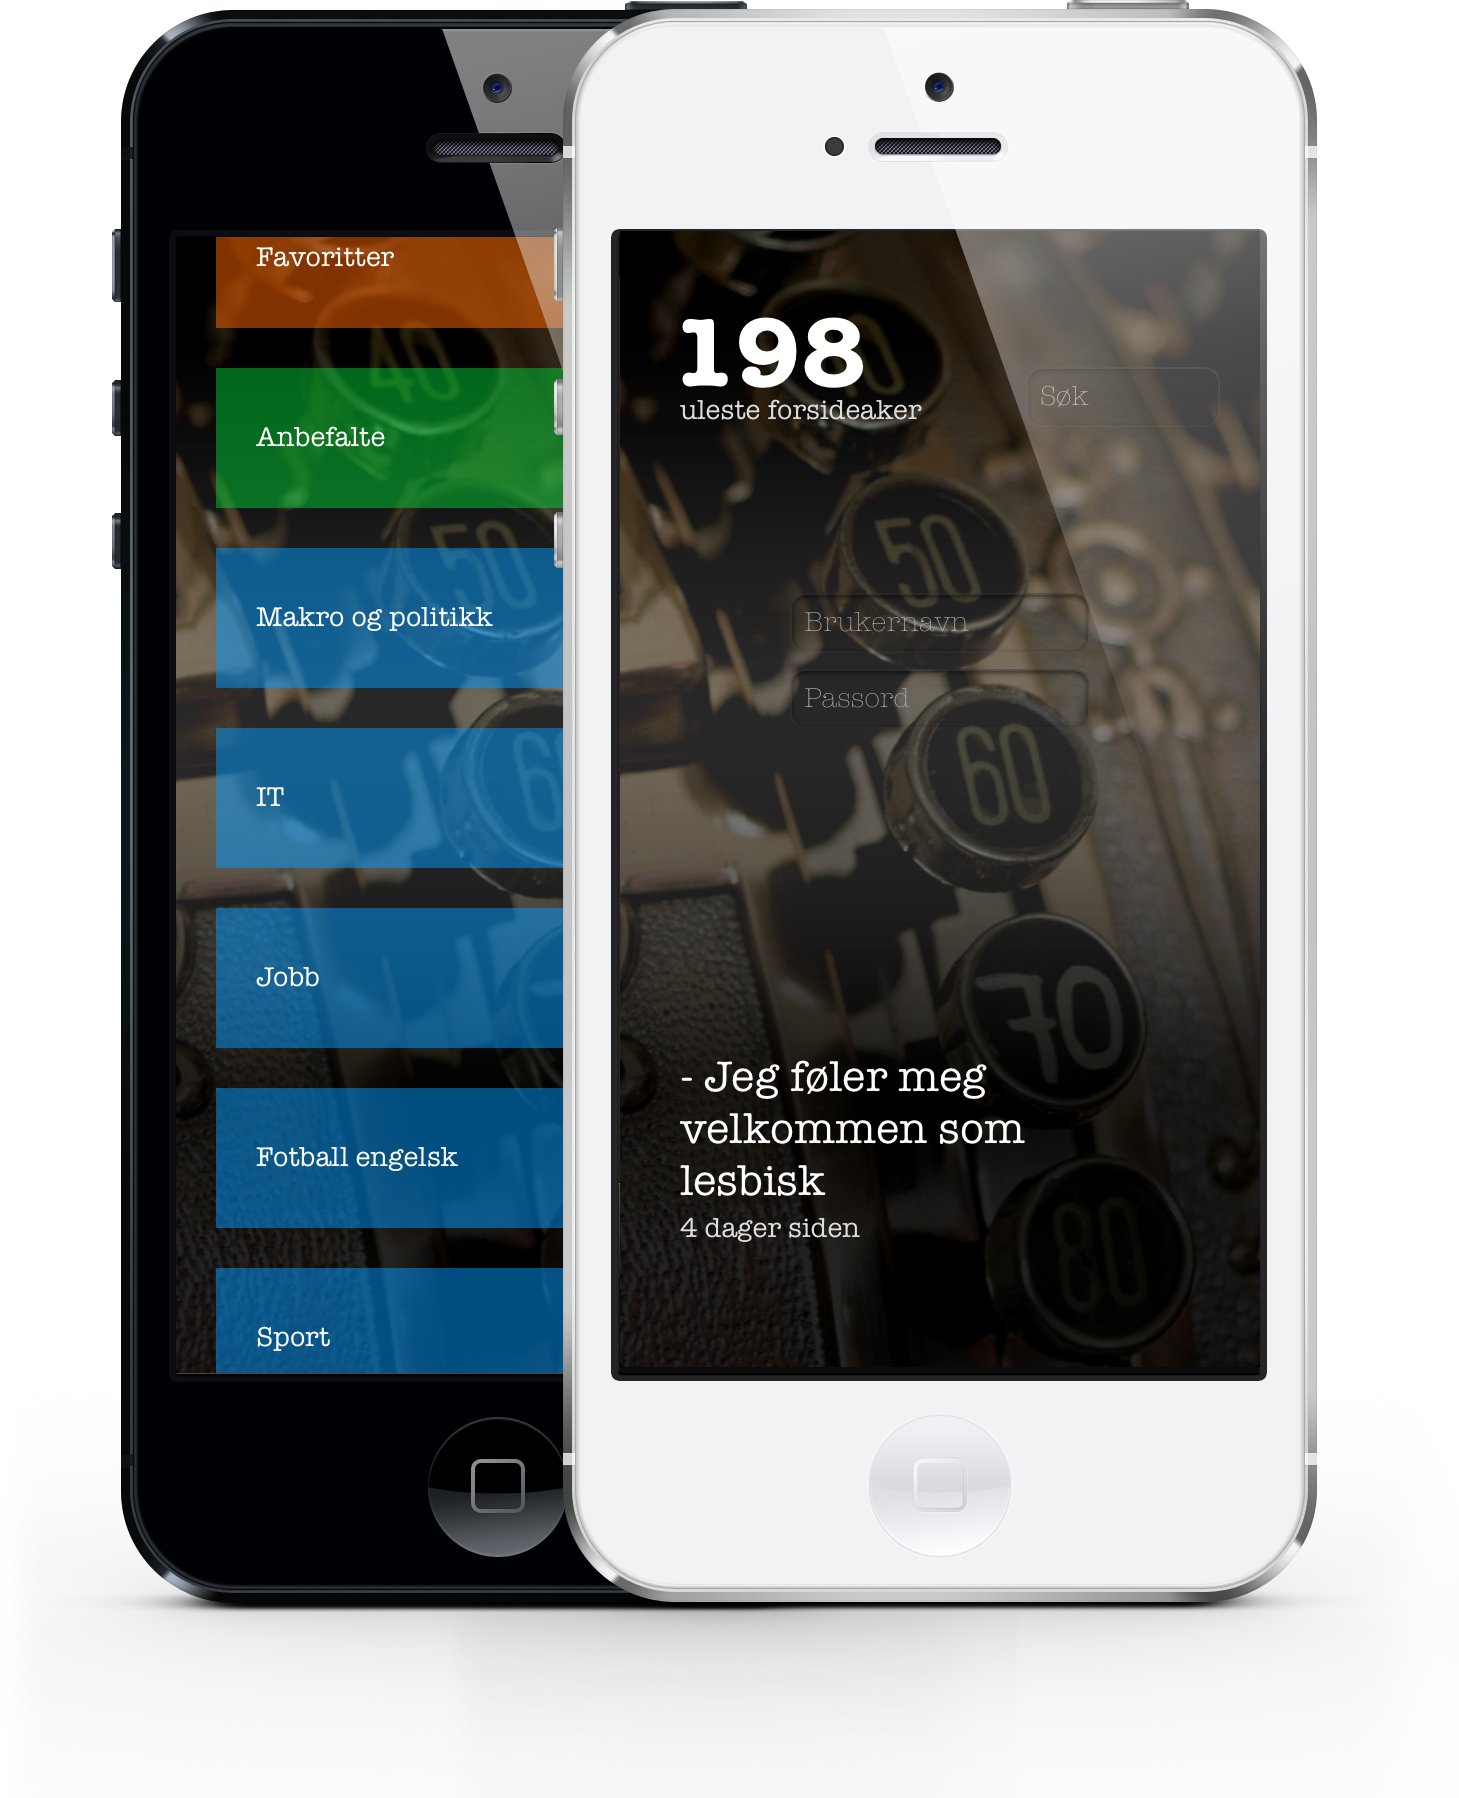
\includegraphics[width=120mm]{GFX/clientApp/categoryAndFrontPage.png}
\caption{Screenshots from the client application showing the start page and the category selection screen.}
\label{screenshots_nyhetene_start_and_category}
\end{figure}

The categories in the category selection screen are categories that are defined by the back-end by analyzing the article's content, as well as the categories set in the RSS feeds provided by the content publishers. The user can also access any stored articles from this menu. By clicking a category in the category selection screen the RSS view will be presented showing the articles from the category clicked. The RSS view is shown in figure \ref{screenshots_nyhetene_rss_and_share}. 

\begin{figure}[!htbp]
\centering
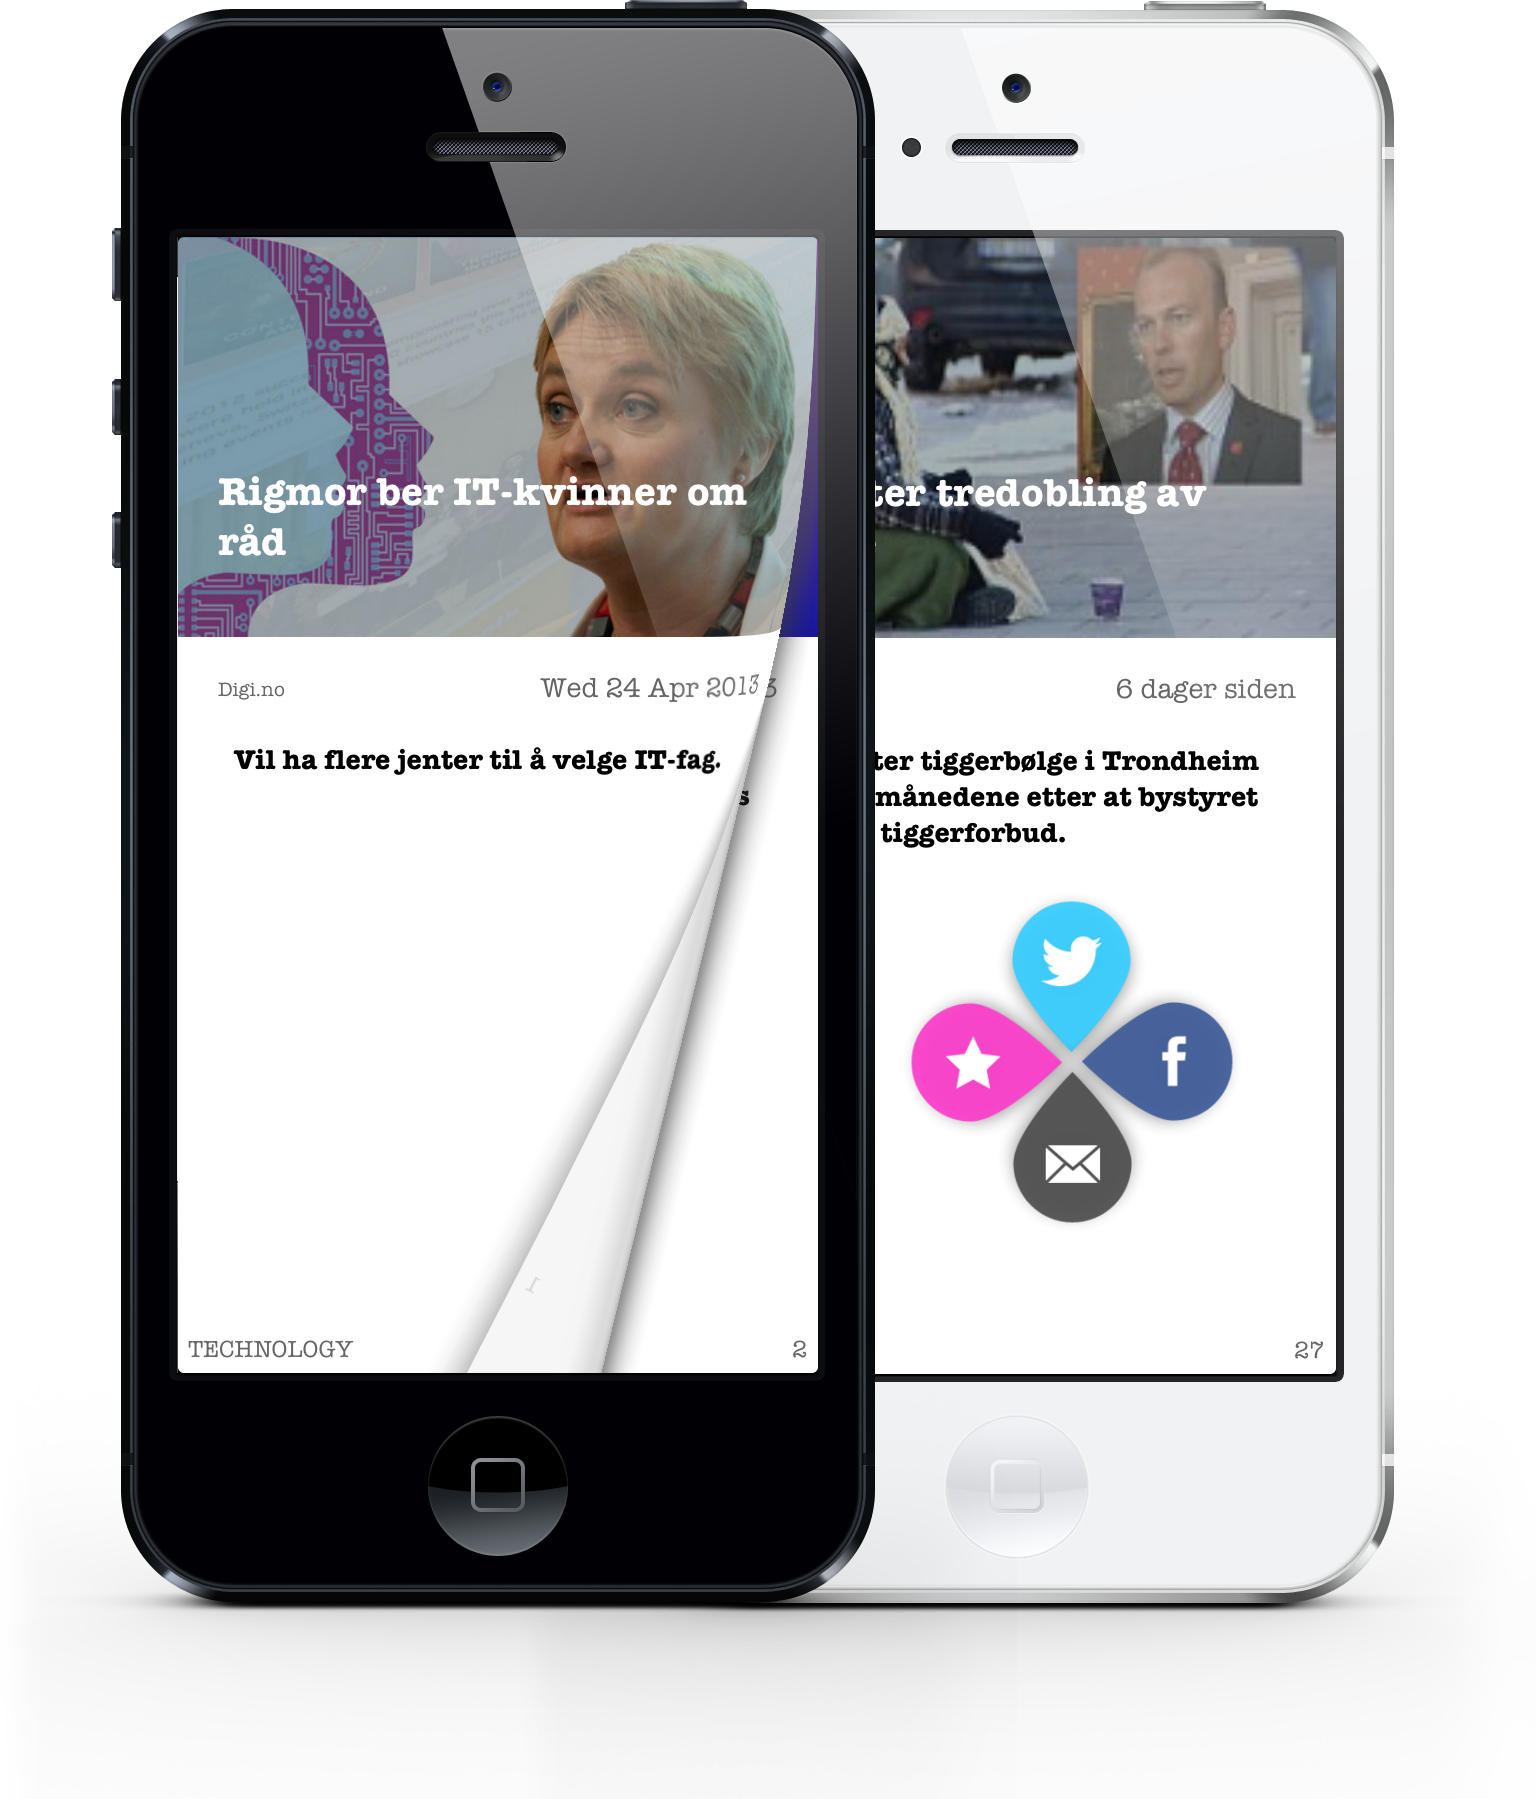
\includegraphics[width=120mm]{GFX/clientApp/rssViewAndShare.png}
\caption{Screenshots from the client application showing the RSS view and the RSS view after triggering the share/save menu.}
\label{screenshots_nyhetene_rss_and_share}
\end{figure}

At the top of the RSS view the title of the article is shown on top of the article's image, if any. The view also shows the publisher, when it was published, which categories the article resides to, the page number the article has of all the articles retrieved in this category and the lead text. To navigate back and forth between the different articles, a horizontal swipe is used. A double tap anywhere on the screen will trigger an update of the news in this category and bring the user to the foremost article. The share/save menu, as shown in the rear image in figure \ref{screenshots_nyhetene_rss_and_share}, is triggered by holding down one finger anywhere on the screen for a short amount of time. From this menu the user can share the article via Facebook, Twitter or mail, as well as storing the article for later reading, by tapping the star icon. By swiping up in this screen the user will be sent back to either the category selection screen or the start screen, depending on which of the two screens triggered the presentation of the RSS view. By swiping down on the RSS view the full article view is presented to the user. The full article view is shown in the foremost image in figure \ref{screenshots_nyhetene_full_article_and_map}


\begin{figure}[!htbp]
\centering
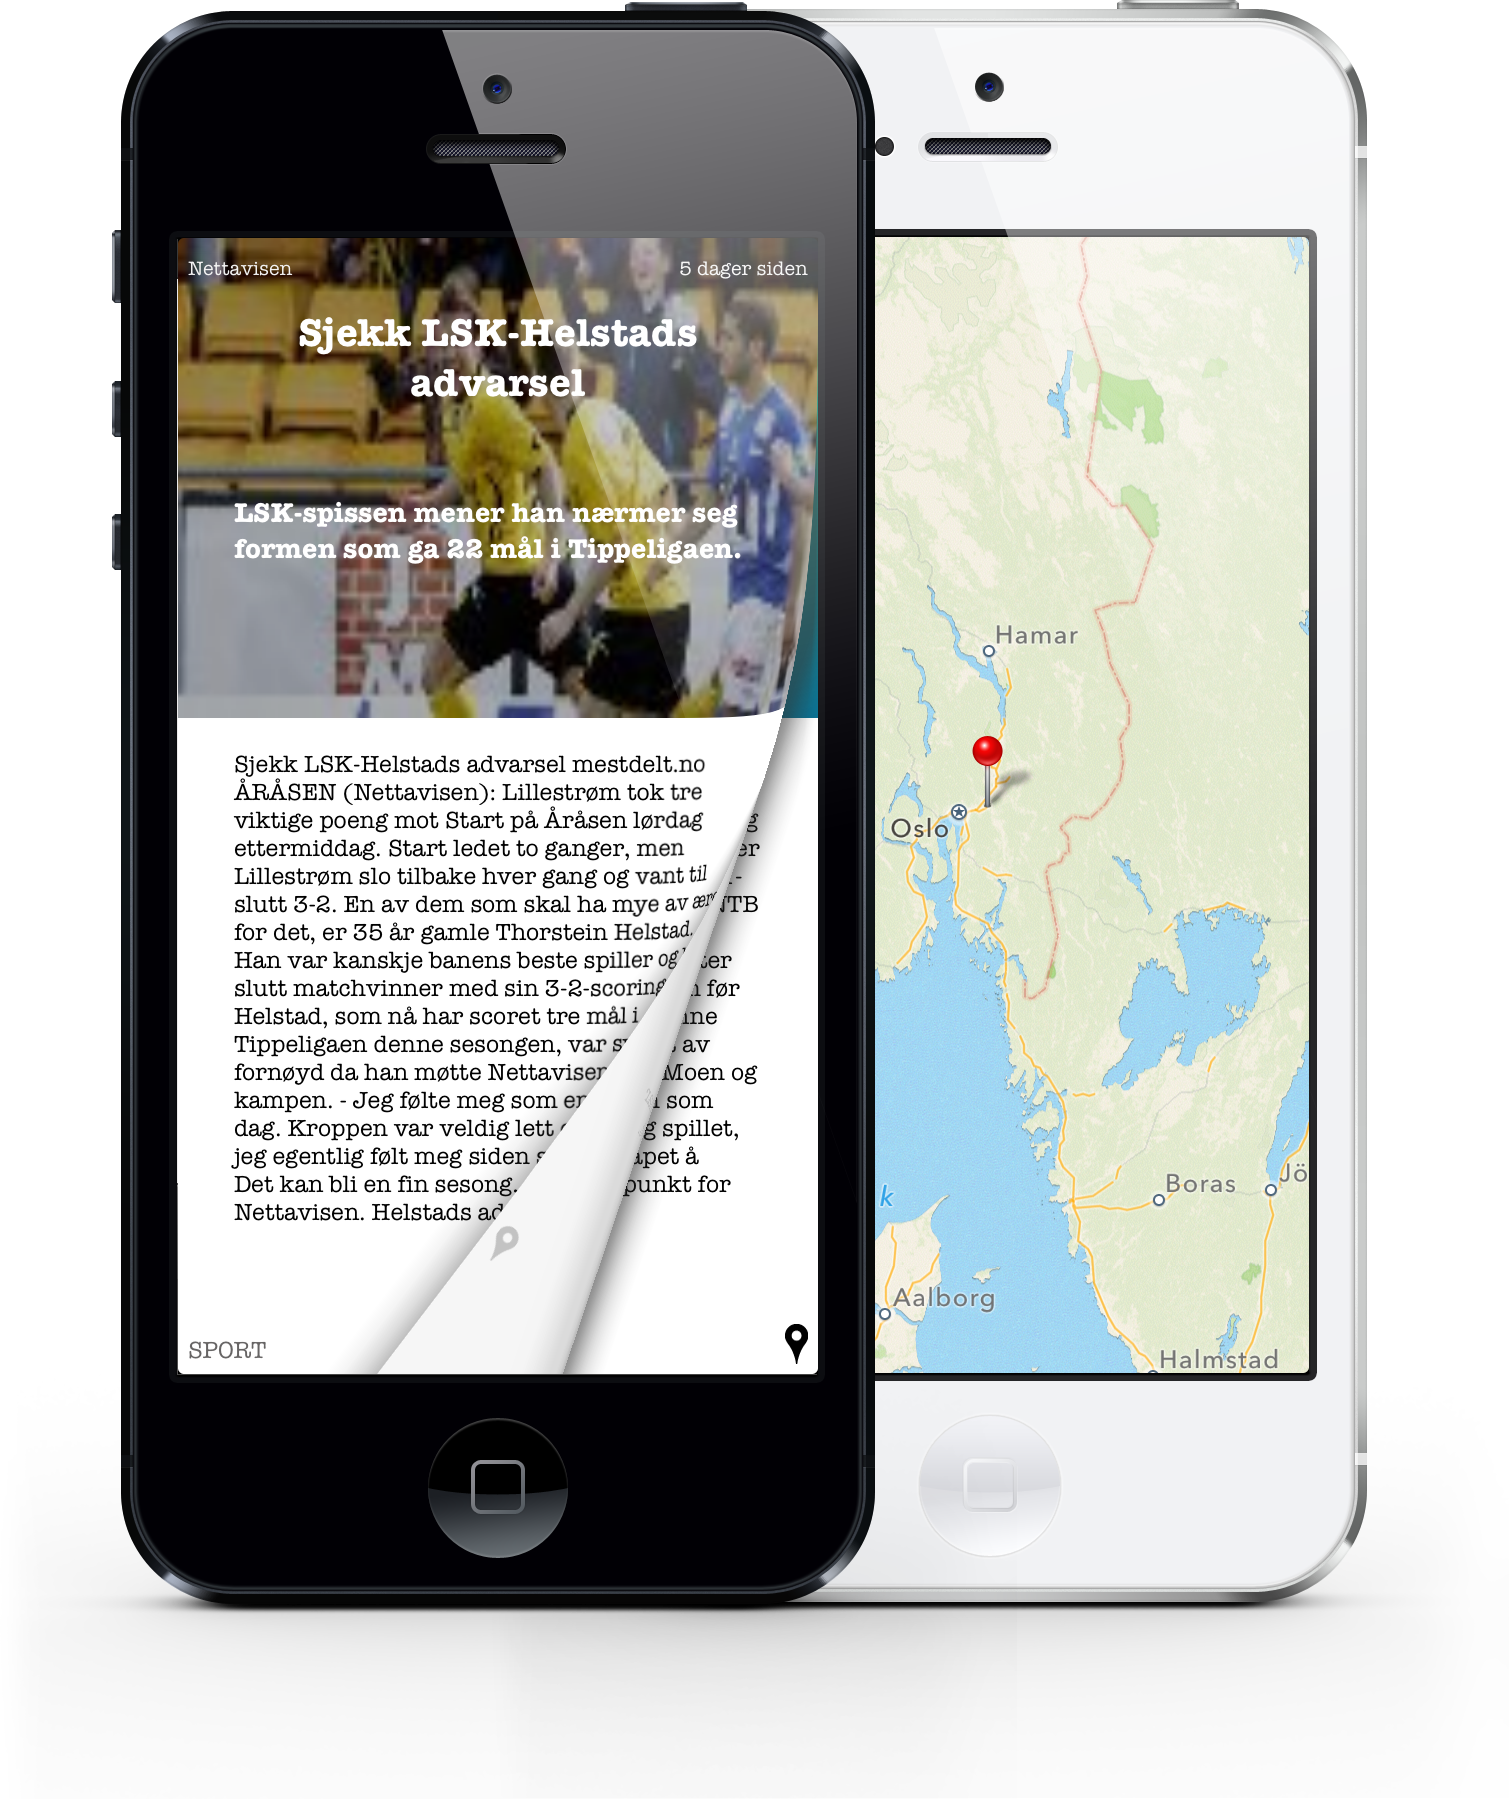
\includegraphics[width=120mm]{GFX/clientApp/swipeForSimilarAndMap.png}
\caption{Screenshots from the client application showing the full article view and the map view.}
\label{screenshots_nyhetene_full_article_and_map}
\end{figure}













\subsection{Technology}